\chapter{Resultados e Discussão}

Como mostrar os resultados de maneira eficiente

\section{resultado parciais}

Afim de validar o método, foram calculados os períodos de um total de $25707$ estrelas variáveis da Grande Nuvem de Magalhães, das quais $3056$ eram Cefeidas clássicas tipo FO e FU, e $22651$ eram RRLyraes tipo AB e C. Os resultado obtidos foram comparados com os resultados do catálogo e o percentual de acertos pode ser visto na tabela \ref{tab:resultados}.

%\begin{center}
%
%\captionof{table}{Quantidade de dados analisados e resultados corretos}
%\begin{tabular}{c|c|c|c} 
%\hline 
%Estrelas & Quantidade & Acertos & Porcentagem \\ 
%\hline 
%Cefeidas & $3056$ & $3048$ & $99.74 \%$ \\ 
%%\hline 
%RRLyraes & $22651$ & $22075$ & $97.46 \%$ \\ 
%\textbf{Total} & $\textbf{25707}$ & $\textbf{25123}$ & $\textbf{97.73 \%}$ \\ 
%\hline 
%\end{tabular} 
%\end{center}


Podemos perceber que para as Cefeidas (estrelas de períodos mais longos) o método apresenta um resultado um pouco melhor se comparado com as RRLyraes (estrelas de período mais curto).


Com estes resultados, podemos confiar no método de entropia condicional, porem, ainda queremos entender melhor o comportamento deste método para dados com diferentes níveis de ruido e com diferentes quantidade de pontos de observação.

\begin{center}
\captionof{table}{Quantidade de dados analisados e resultados corretos}
\begin{tabular}{c|c|c|c} 
\hline 
Estrelas & Quantidade & Acertos & Porcentagem \\ 
\hline 
Cefeidas FU & $1818$ & $1817$ & $99,94 \%$ \\ 
Cefeidas FO & $1238$ & $1231$ & $99,43 \%$ \\ 
%\hline 
RRLyraes AB& $17693$ & $17540$ & $99,14 \%$ \\ 
RRLyraes C& $4958$ & $4535$ & $91,47 \%$ \\ 
\textbf{Total} & $\textbf{25707}$ & $\textbf{25123}$ & $\textbf{97,73 \%}$ \\ 
\hline 
\end{tabular} 
\label{tab:resultados}
\end{center}


\subsection{Dados Sintéticos}

Dados sintéticos foram criados a fim de explorar o método e entender até onde podemos utiliza-lo. De acordo com a tabela \ref{tab:resultados}, as RRLyraes apresentaram uma taxa menor de acerto então elas foram utilizadas como referencia para construir os dados sintéticos. Assim, foi determinado a partir dos dados qual a variação média entre os pontos de observação para assim calcular a amostragem média dos dados. A amostragem representa a frequência de pontos de observação. Desta forma, foi calculado a amostragem,
\begin{align}
f_s = \frac{1}{dt} = 0.1473 .
\end{align}

Obtendo a amostragem, podemos construir dados sintéticos variando a amostragem e o nível de ruído afim de estudar o comportamento do método. De acordo com \cite{ce} e \cite{entropy}, para construir dados sintéticos semelhantes com os dados observacionais da maioria dos Surveys de estrelas variáveis, podemos utilizar a seguinte expressão,
\begin{align}
m(t) &= A_0 + \sum_i^3 A_n \sin \Big( \frac{2 n \pi t}{P} \Big) + \varepsilon \eta
\end{align}
em que \(\varepsilon\) é um fator de escala para o ruido entre \(0.0\) e \(1.0\), \(\eta\) é uma distribuição gaussiana com média zero e desvio unitário e \(P\) é o período médio das RRlyraes que, segundo \cite{lyraes} é de \(0.576\) dias.

A influencia da amostragem está no vetor \(t\) que é construindo a fim de representar de forma mais fiel possível os dados do Catálogo OGLE-III. Sendo assim, o vetor tempo é construído com os seguinte parâmetros: tempo inicial de \(2152.5019\) HJD, tempo final de \(4539.4593\) HJD e espaçamento entre os pontos \(dt = 1 / f\) em que \(f = n \times f_s\) e \(n\) é um parâmetro de escala para a amostragem. Os tempos iniciais e finais foram escolhidos desta forma por serem os valores de maior frequência entre os dados das RRLyraes. Quatro exemplos de curva de luz sintética gerada pelo método acima podem ser vistas na figura \ref{fig:exemplo_curva_luz}. 

\begin{figure}[H]
\centering
\begin{subfigure}{.5\textwidth}
  \centering
  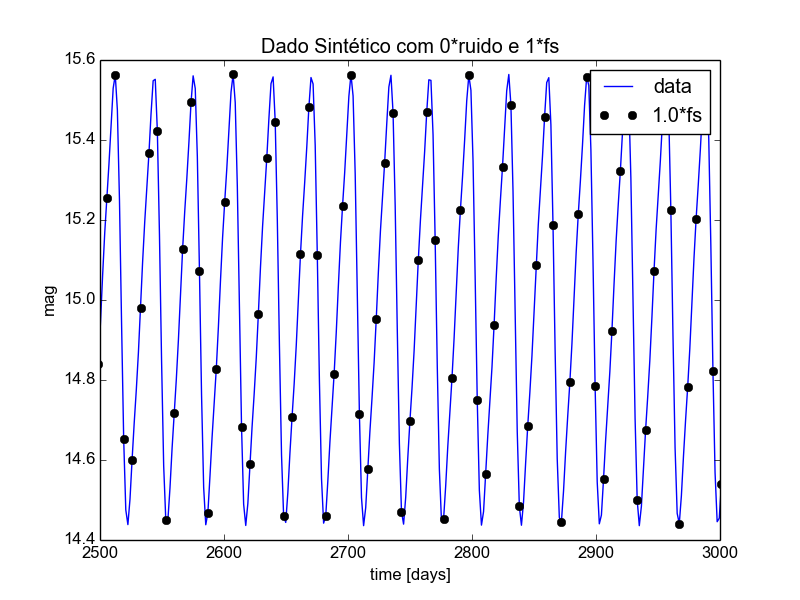
\includegraphics[width=\linewidth]{dado_sintetico_0_ruido_1_amos.png}
  \caption{Dado sem ruído e com amostragem padrão}
  \label{fig:1amos}
\end{subfigure}%
\begin{subfigure}{.5\textwidth}
  \centering
  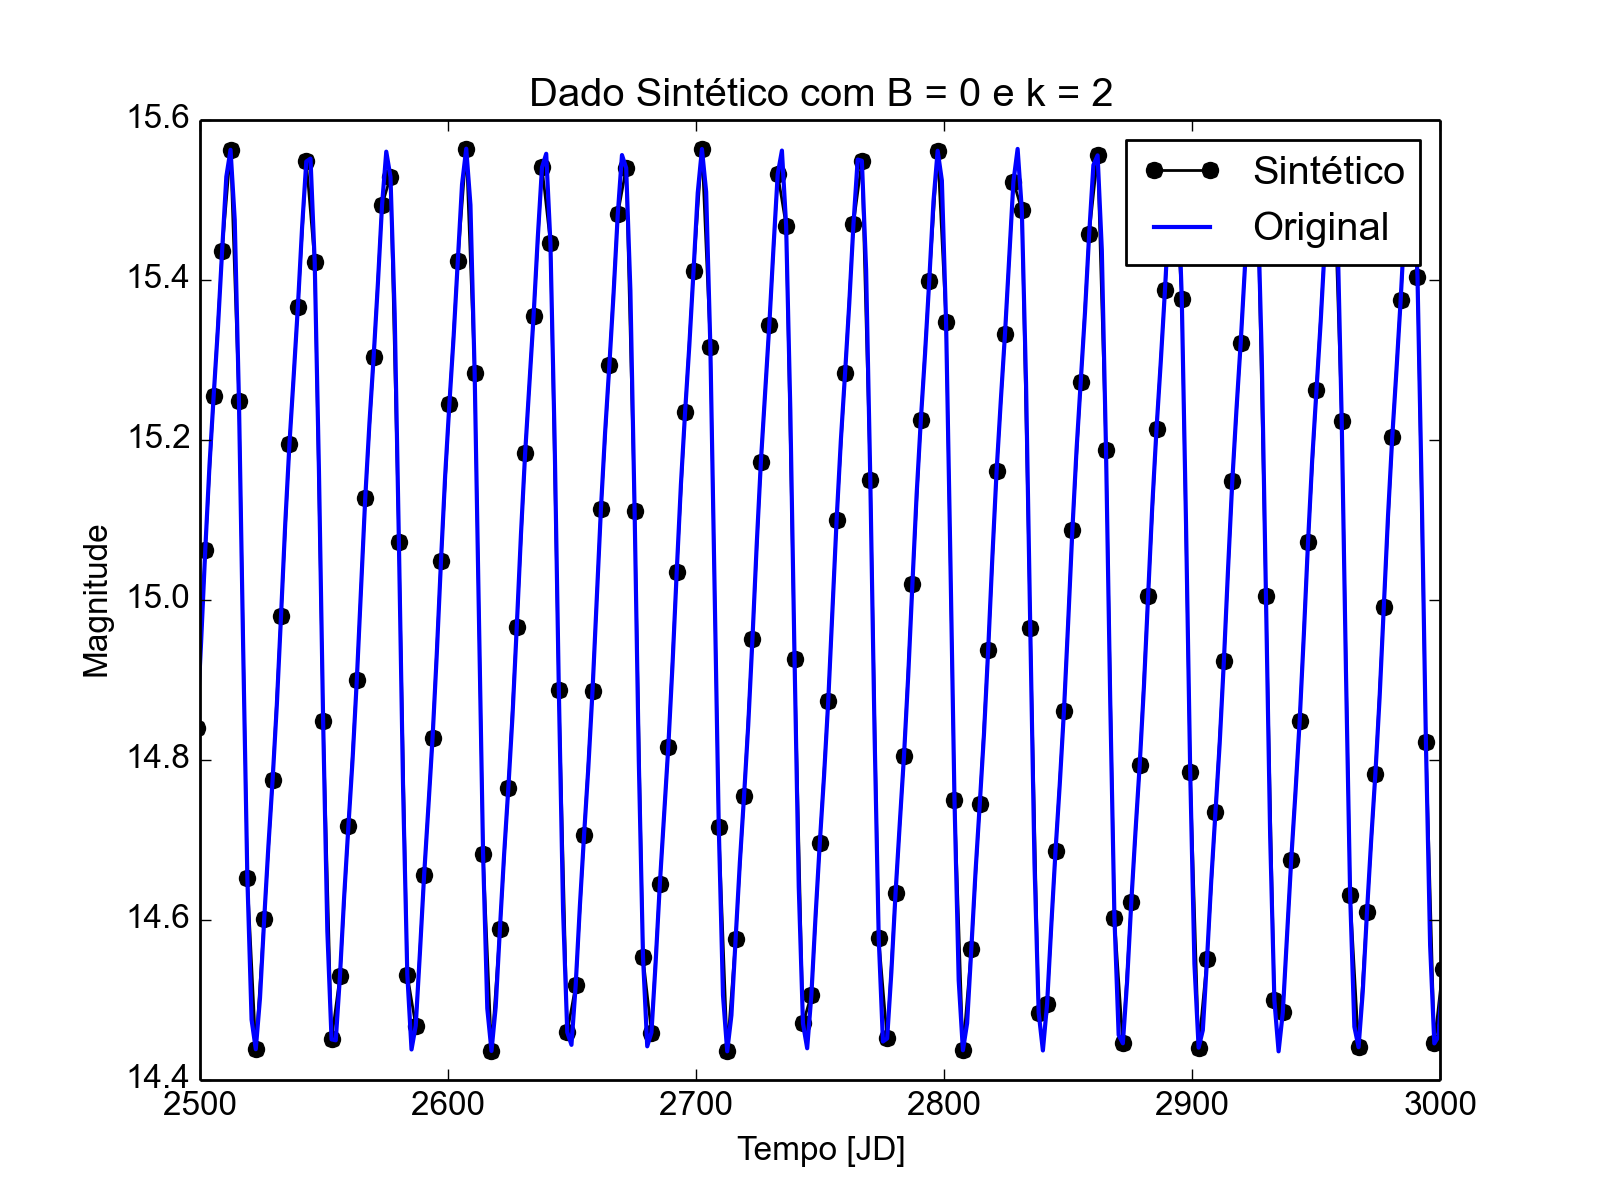
\includegraphics[width=\linewidth]{dado_sintetico_0_ruido_2_amos.png}
  \caption{Dado sem ruído com $n=2$}
  \label{fig:2amos}
  \end{subfigure}
\\
\begin{subfigure}{.5\textwidth}
  \centering
  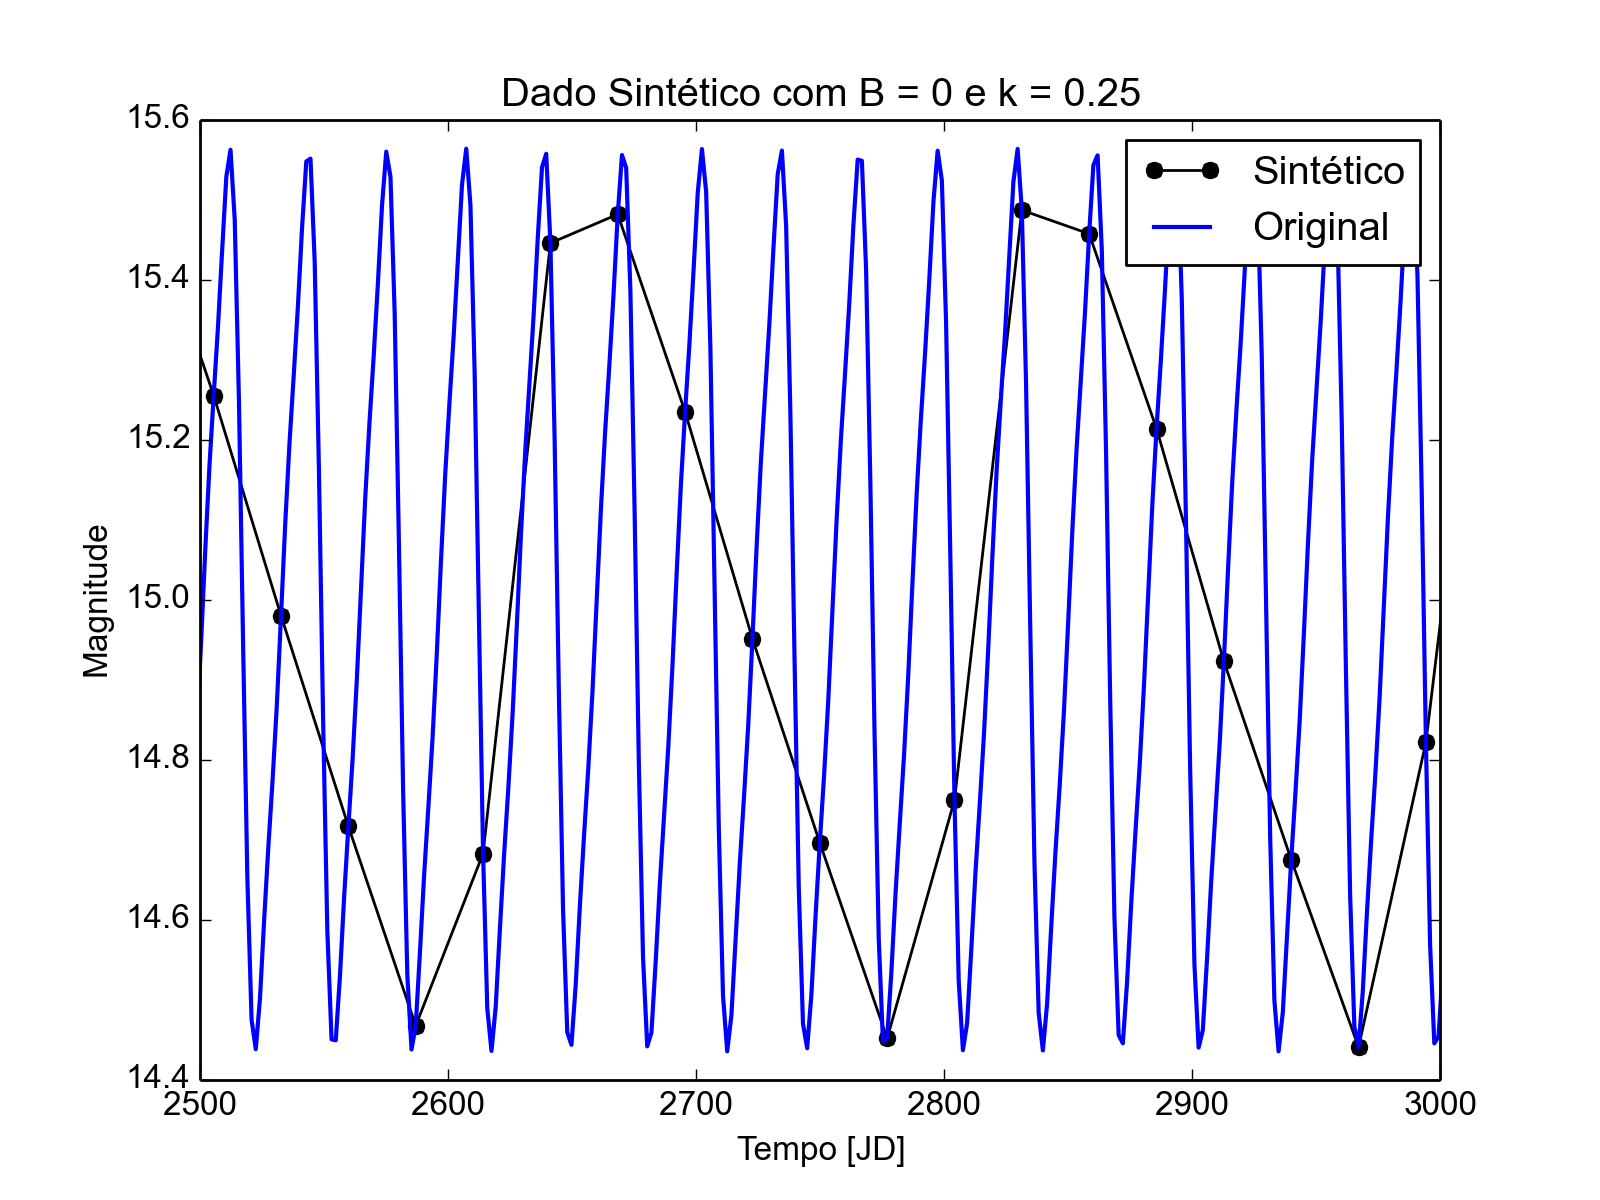
\includegraphics[width=\linewidth]{dado_sintetico_0_ruido_0_25_amos.png}
  \caption{Dado sem ruído e com $n=1/4$}
  \label{fig:025amos}
\end{subfigure}%
\begin{subfigure}{.5\textwidth}
  \centering
  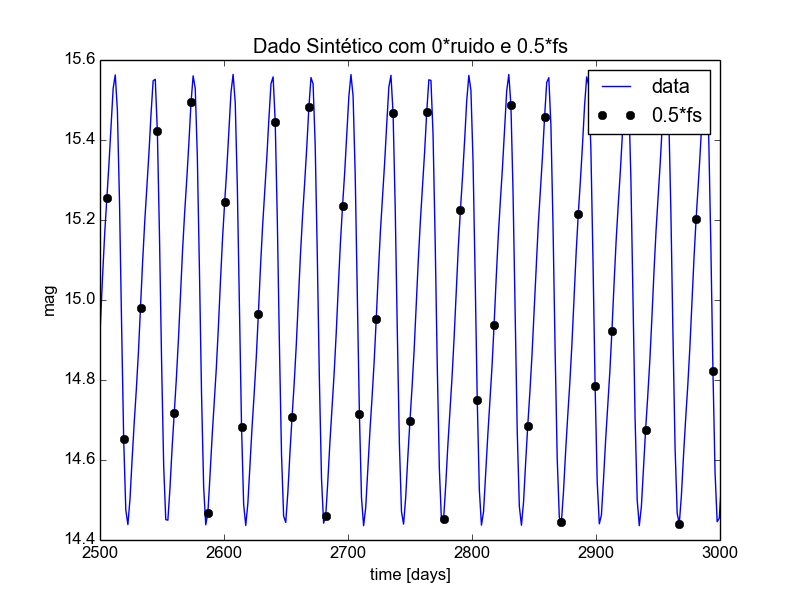
\includegraphics[width=\linewidth]{dado_sintetico_0_ruido_0_5_amos.png}
  \caption{Dado sem ruído com $n=1/2$}
  \label{fig:05amos}
  \end{subfigure}
\caption{Exemplos curva de luz sintética}
\label{fig:exemplo_curva_luz}
\end{figure}

Na figura \ref{fig:exemplo_curva_luz}, os ponto pretos são os pontos de observação e a linha contínua é o dado original com \(n=1\). Podemos perceber que quanto maior a amostragem, maior a quantidade de pontos, assim o método aplicado a um dado com uma grande amostragem deve retornar um período com maior precisão do que comparado à um dado com pequena amostragem.

Então, para estudar a influencia da amostragem nos dados, foram gerados dados sintéticos variando o parâmetro \(n\) da amostragem de $0.25$ a $4$ com intervalo de $0.25$ e variando o fator de escala $\varepsilon$ de $0.0$ até $1.0$ com intervalo de $0.05$ assim obtendo $300$ curvas de luz. No momento, estamos pensando em como demonstrar os resultados obtidos. Uma forma para demonstrar os dados é fazendo um mapa de cor entre ruído e amostragem onde a cor representa o valor \(|(P - P_0)/P_0|\), ou seja, quanto que o período calculado está variando em relação ao período original. O mapa de cor é feito em escala de cinza, em que a cor mais escura representa o valor 0 (período calculado = período real) e quanto mais clara a cor, maior o desvio do período.	%o período calculado menos o período real do sinal dividido pelo período real, em  uma escala de cinza.

\begin{figure}[H]
\centering
\hspace{-2.5cm}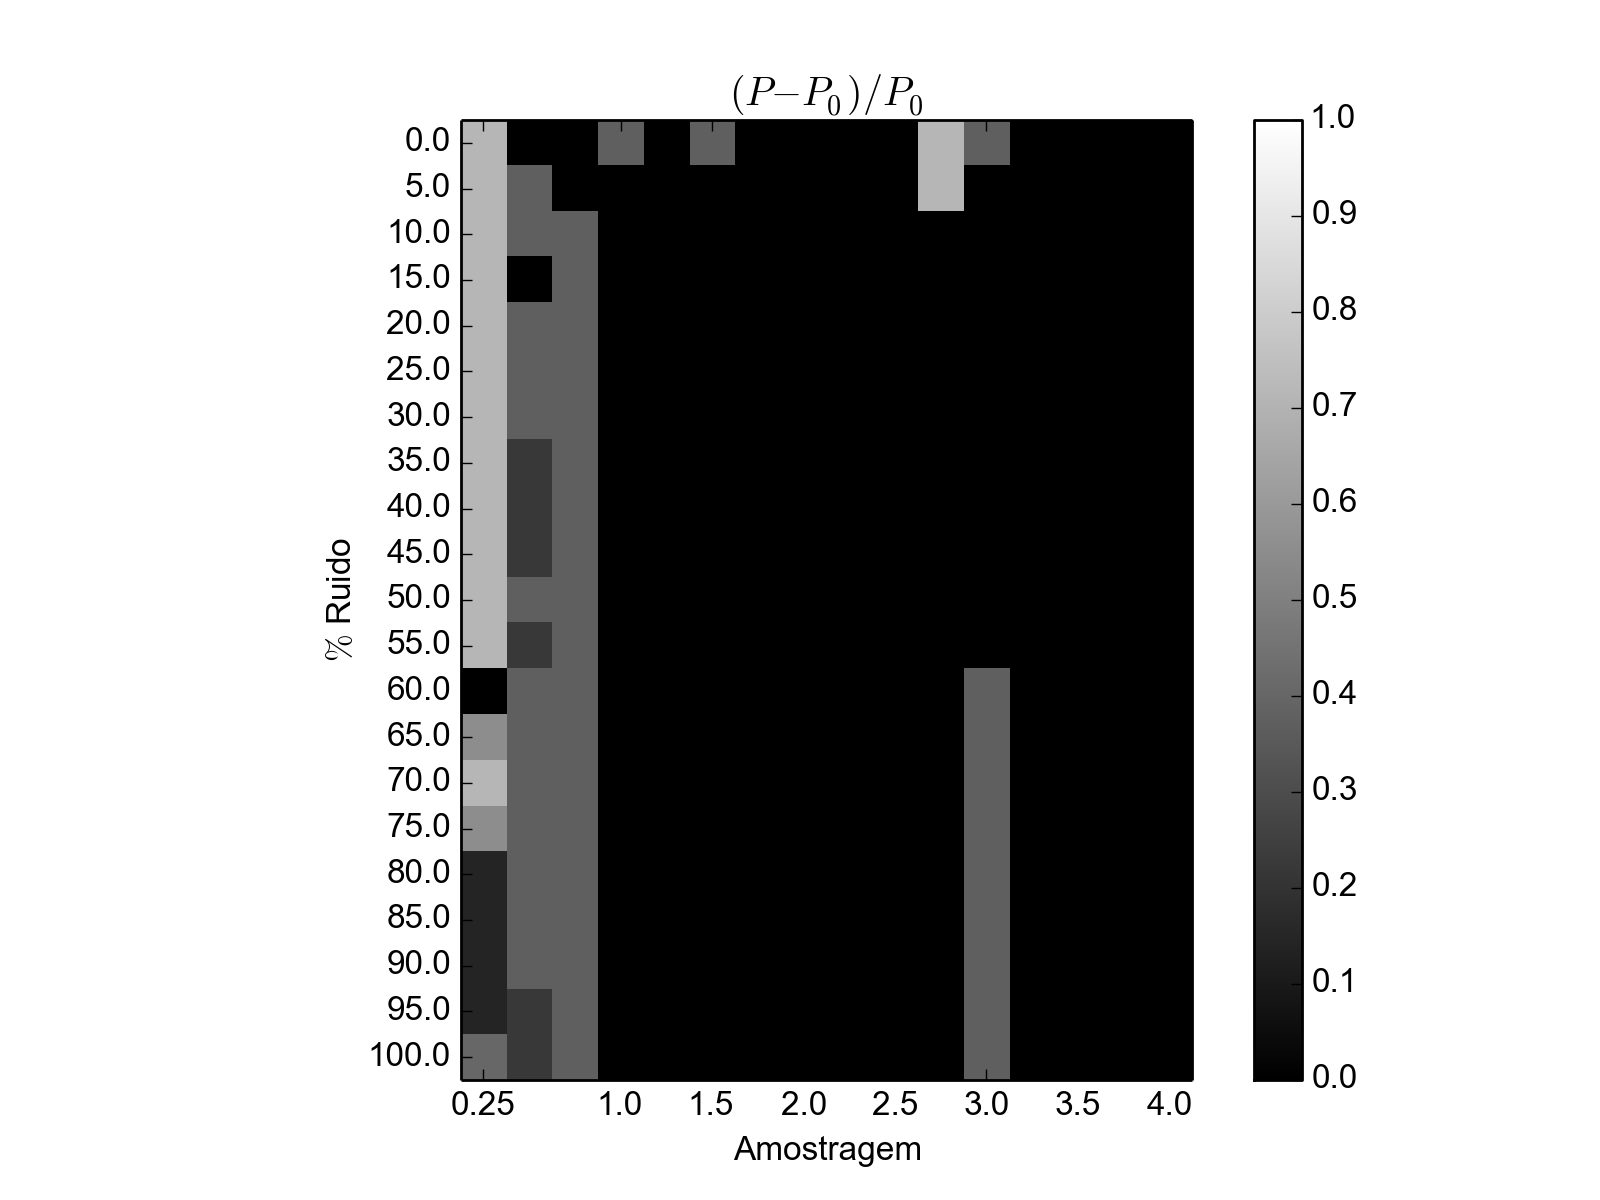
\includegraphics[scale=.8]{ce_inshow.png}
\label{fig:imshow}
\caption{Resultados obtidos em escala de cinza}
\end{figure}

Os valores iguais a zero (cor preta) representam as configurações em que o método de entropia condicional calculou o período corretamente.

Com esta análise, é possível construir uma ferramenta que nos indica como os dados influenciam no resultado do método, ou ainda, partindo do resultado que se espera obter, é possível escolher como a observação deve ser feita.